%%%%%%%%%%%%%%%%%%%%%%%%%%%%%%%%%%%%%%%%%%%%%%%%%%%%%%%%%%%%%%%%%%%%%%%%%%%%%%%%%%%%%%%%%%%%%%%%%%%%%%%%%%%%%%%%%%%%%%%%%%%%%%%%%%%%%%%%%%%%%%%%%%%%%%%%%%%%%%%%%%%%%%%%%%%%%%%%%%%%%%%%%%%%
% Written By Michael Brodskiy
% Class: Linear Algebra
% Professor: L. Knight
%%%%%%%%%%%%%%%%%%%%%%%%%%%%%%%%%%%%%%%%%%%%%%%%%%%%%%%%%%%%%%%%%%%%%%%%%%%%%%%%%%%%%%%%%%%%%%%%%%%%%%%%%%%%%%%%%%%%%%%%%%%%%%%%%%%%%%%%%%%%%%%%%%%%%%%%%%%%%%%%%%%%%%%%%%%%%%%%%%%%%%%%%%%%

\documentclass[12pt]{article} 
\usepackage{alphalph}
\usepackage[utf8]{inputenc}
\usepackage[russian,english]{babel}
\usepackage{titling}
\usepackage{amsmath}
\usepackage{graphicx}
\usepackage{enumitem}
\usepackage{amssymb}
\usepackage{physics}
\usepackage{tikz}
\usepackage{mathdots}
\usepackage{yhmath}
\usepackage{cancel}
\usepackage{color}
\usepackage{siunitx}
\usepackage{array}
\usepackage{multirow}
\usepackage{gensymb}
\usepackage{tabularx}
\usepackage{booktabs}
\usetikzlibrary{fadings}
\usetikzlibrary{patterns}
\usetikzlibrary{shadows.blur}
\usetikzlibrary{shapes}
\usepackage[super]{nth}
\usepackage{expl3}
\usepackage[version=4]{mhchem}
\usepackage{hpstatement}
\usepackage{rsphrase}
\usepackage{everysel}
\usepackage{ragged2e}
\usepackage{geometry}
\usepackage{fancyhdr}
\usepackage{cancel}
\usepackage{multicol}
\geometry{top=1.0in,bottom=1.0in,left=1.0in,right=1.0in}
\newcommand{\subtitle}[1]{%
  \posttitle{%
    \par\end{center}
    \begin{center}\large#1\end{center}
    \vskip0.5em}%

}
\usepackage{hyperref}
\hypersetup{
colorlinks=true,
linkcolor=blue,
filecolor=magenta,      
urlcolor=blue,
citecolor=blue,
}

\urlstyle{same}


\title{Linear Algebra 1.1 Homework}
\date{}
\author{Michael Brodskiy\\ \small Instructor: Prof. Knight}

% Mathematical Operations:

% Sum: $$\sum_{n=a}^{b} f(x) $$
% Integral: $$\int_{lower}^{upper} f(x) dx$$
% Limit: $$\lim_{x\to\infty} f(x)$$

\begin{document}

\maketitle

\begin{enumerate}

    \setcounter{enumi}{2}

  \item Not linear

    \setcounter{enumi}{4}

  \item Not linear

    \setcounter{enumi}{8}

  \item 

    \begin{equation*}
      \begin{split}
        y&\rightarrow s\\
        z&\rightarrow t\\
        S&=\left\{ (1-s-t,s,t) \right\}
      \end{split}
      \label{1}
    \end{equation}

  \item

    \begin{equation*}
      \begin{split}
        x_2&\rightarrow s\\
        x_3&\rightarrow t\\
        S&=\left\{ (1-2s+3t,s,t) \right\}
      \end{split}
      \label{2}
    \end{equation}

  \item \textbf{ }

    \begin{multicols}{2}

      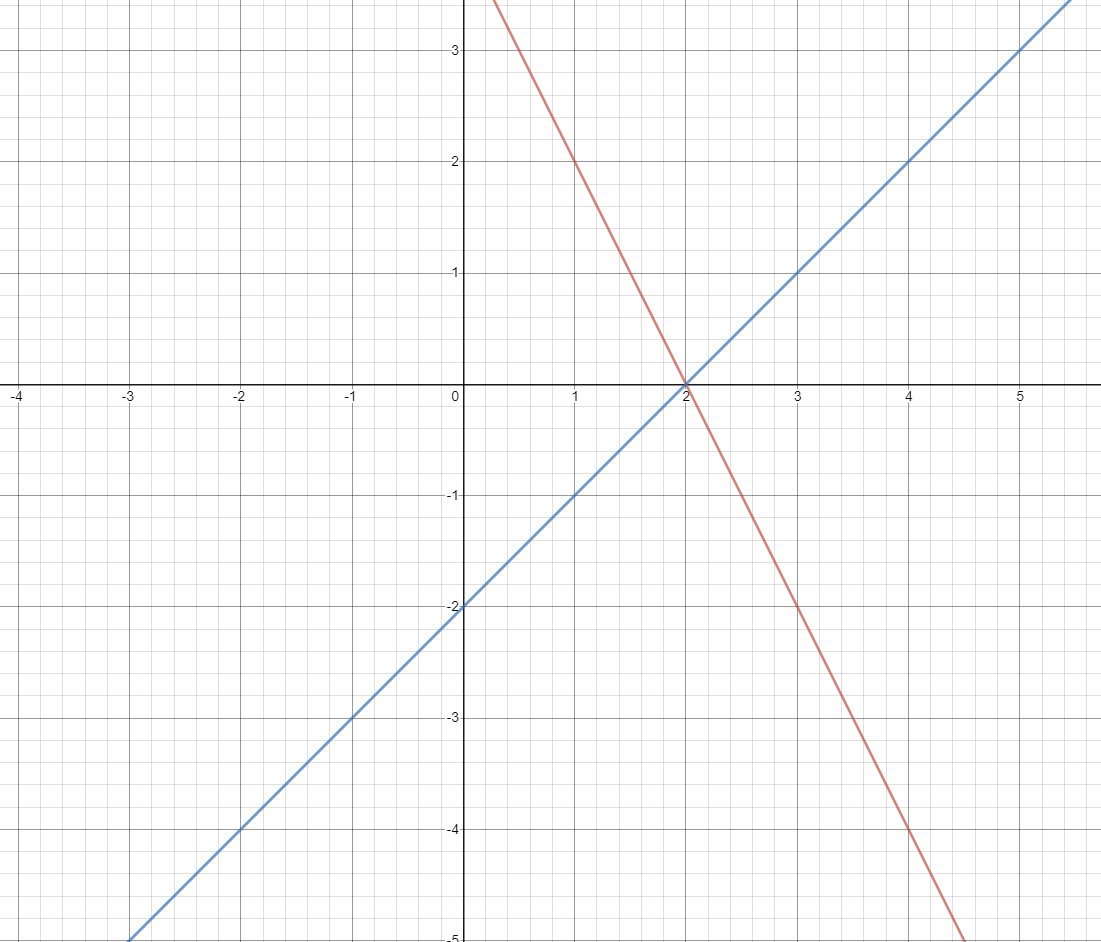
\includegraphics[width=.5\textwidth]{Figures/Prob11Graph.png}

    \begin{equation*}
      \begin{split}
        \begin{array}{l l}
          2x+y=4 & L_1\\
          x-y=2 & L_2
        \end{array}\\
        L_1-L_2\rightarrow x=2\\
        2(2)+y=4\\
        y=0\\
        \text{The solution is at point } (2,0)
      \end{split}
      \label{3}
    \end{equation}

  \end{multicols}

    \setcounter{enumi}{12}

  \item \textbf{ }

    \begin{multicols}{2}

      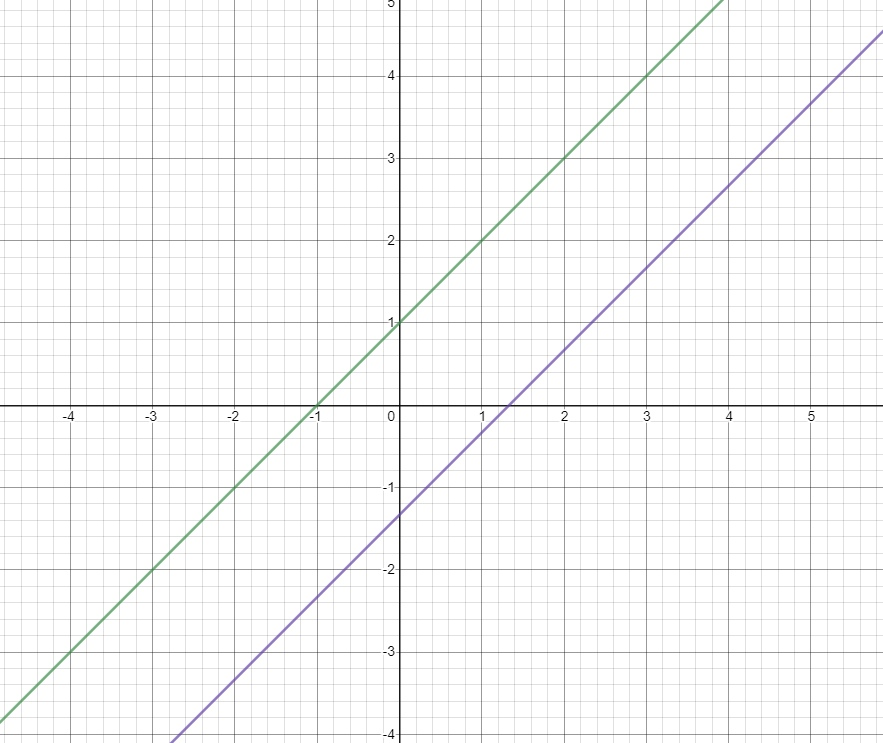
\includegraphics[width=.5\textwidth]{Figures/Prob13Graph.png}

    \begin{equation*}
      \begin{split}
        \begin{array}{l l}
          -x+y=1 & L_1\\
          3x-3y=4 & L_2
        \end{array}\\
        -\frac{1}{3}L_2\rightarrow -x+y=-\frac{4}{3}\\
        \text{No Solution, Lines Parallel}
      \end{split}
      \label{4}
    \end{equation}

  \end{multicols}

    \setcounter{enumi}{14}

  \item \textbf{ }

    \begin{multicols}{2}

      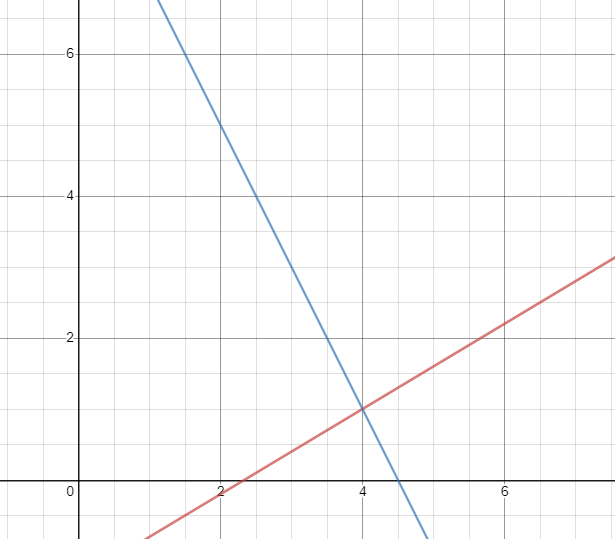
\includegraphics[width=.5\textwidth]{Figures/Prob15Graph.png}

    \begin{equation*}
      \begin{split}
        \begin{array}{l l}
          3x-5y=7 & L_1\\
          2x+y=9 & L_2
        \end{array}\\
        5L_2+L_1\rightarrow 13x=52\\
        x=4\\
        2(4)+y=9\\
        y=1\\
        \text{The solution is at point } (4,1)
      \end{split}
      \label{5}
    \end{equation}

  \end{multicols}

  \newpage

    \setcounter{enumi}{16}

  \item \textbf{ }

    \begin{multicols}{2}

      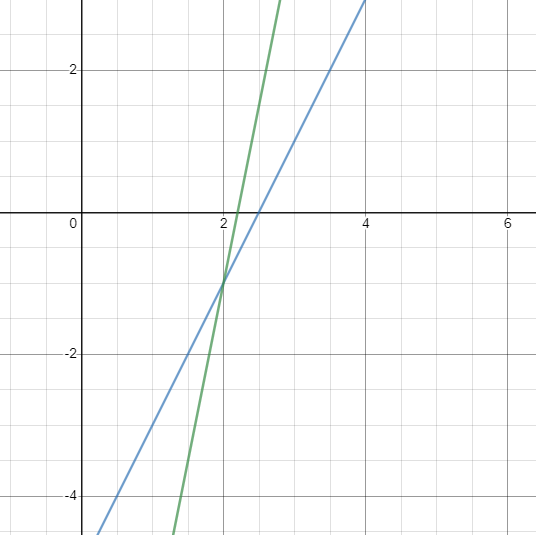
\includegraphics[width=.5\textwidth]{Figures/Prob17Graph.png}

    \begin{equation*}
      \begin{split}
        \begin{array}{l l}
          2x-y=5 & L_1\\
          5x-y=11 & L_2
        \end{array}\\
        L_2-L_1\rightarrow 3x=6\\
        x=2\\
        2(2)-y=5\\
        y=-1\\
        \text{The solution is at point } (2,-1)
      \end{split}
      \label{6}
    \end{equation}

  \end{multicols}

    \setcounter{enumi}{18}

  \item \textbf{ }

    \begin{multicols}{2}

      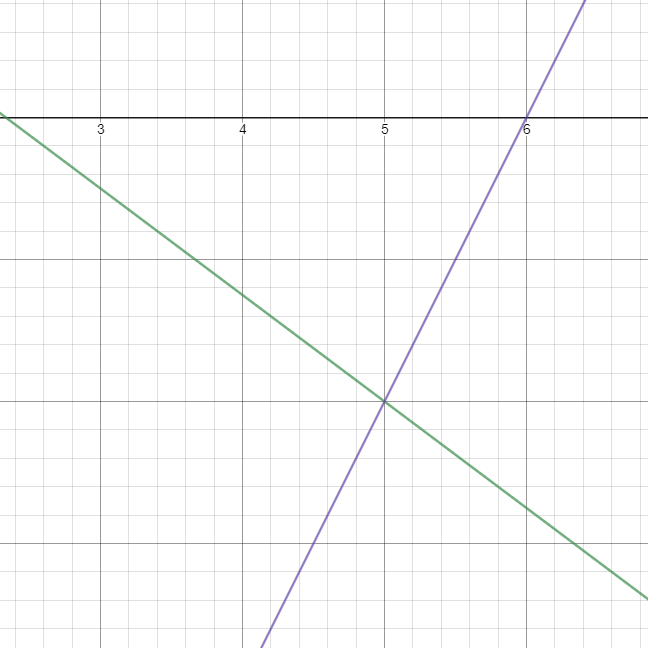
\includegraphics[width=.5\textwidth]{Figures/Prob19Graph.png}

    \begin{equation*}
      \begin{split}
        \begin{array}{l l}
          \frac{x+3}{4}+\frac{y-1}{3}=1 & L_1\\
          2x-y=12 & L_2
        \end{array}\\
        12L_1\rightarrow 3x+4y=7\\
        4L_2+(3x+4y=7)\rightarrow 11x=55\\
        x=5\\
        2(5)-y=12\\
        y=-2\\
        \text{The solution is at point } (5,-2)
      \end{split}
      \label{7}
    \end{equation}

  \end{multicols}

  \newpage

    \setcounter{enumi}{20}

  \item \textbf{ }

    \begin{multicols}{2}

      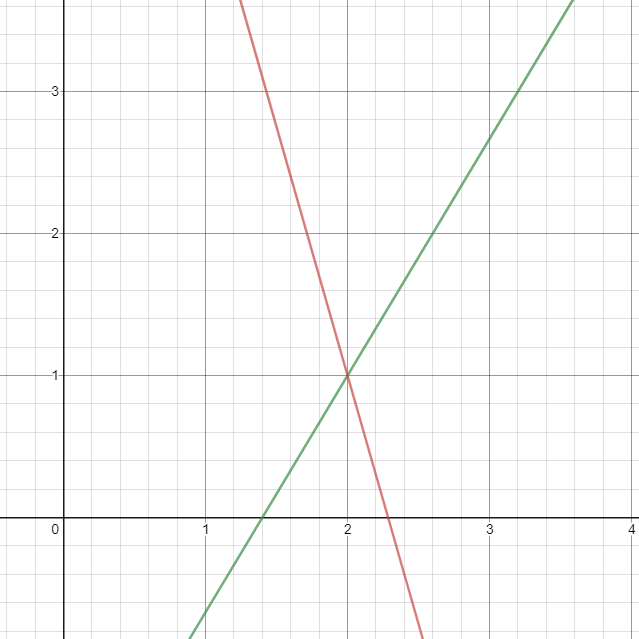
\includegraphics[width=.5\textwidth]{Figures/Prob21Graph.png}

    \begin{equation*}
      \begin{split}
        \begin{array}{l l}
          .05x-.03y=.07 & L_1\\
          .07x+.02y=.16 & L_2
        \end{array}\\
        200L_1+300L_2\rightarrow 31x=62\\
        x=2\\
        .05(2)-.03y=.07\\
        y=1\\
        \text{The solution is at point } (2,1)
      \end{split}
      \label{8}
    \end{equation}

  \end{multicols}

    \setcounter{enumi}{22}

  \item \textbf{ }

    \begin{multicols}{2}

      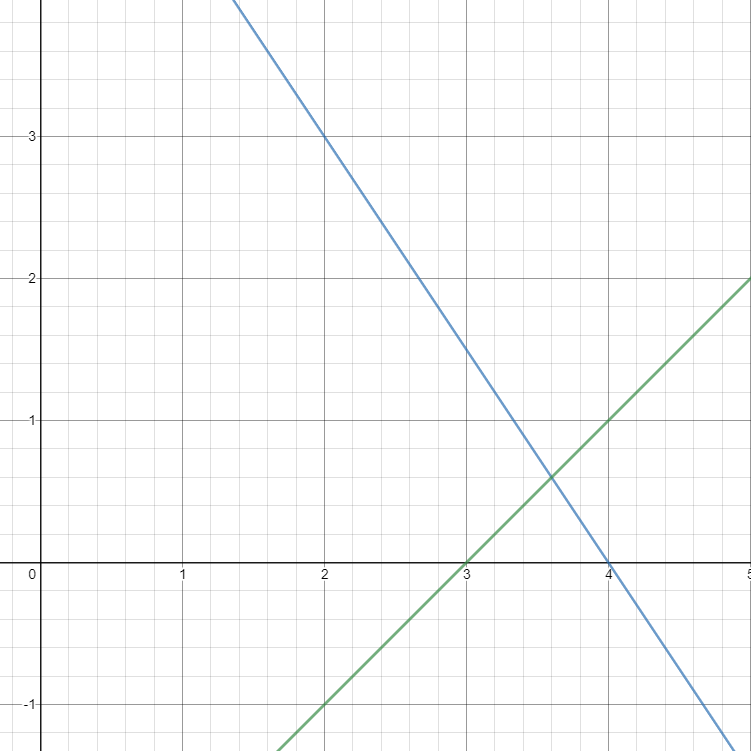
\includegraphics[width=.5\textwidth]{Figures/Prob23Graph.png}

    \begin{equation*}
      \begin{split}
        \begin{array}{l l}
          \frac{x}{4} + \frac{y}{6} = 1 & L_1\\
          x-y=3 & L_2
        \end{array}\\
        24L_1\rightarrow 6x+4y=24\\
        4L_2+(6x+4y=24)\rightarrow 10x=36\\
        x=3.6\\
        -y=3-3.6\\
        y=.6\\
        \text{The solution is at point } (3.6,0.6)
      \end{split}
      \label{9}
    \end{equation}

  \end{multicols}

    \setcounter{enumi}{24}

  \item $\begin{array}{|r|} \hline x_1-x_2=2\\ x_2=3\\ \hline \end{array} \rightarrow x_1=2+3 \rightarrow x_1=5$

    \begin{equation*}
      S=\left\{ (5,3) \right\}
      \label{10}
    \end{equation}

    \setcounter{enumi}{26}

  \item $\begin{array}{|r|} \hline -x+y-z=0\\ 2y+z=3\\ \frac{1}{2}z=0\\ \hline\end{array} \rightarrow z=0 \rightarrow 2y=3 \rightarrow y=\frac{3}{2} \rightarrow -x=-\frac{3}{2}\rightarrow x=\frac{3}{2}$

    \begin{equation*}
      S=\left\{ \frac{3}{2},\frac{3}{2},0 \right\}
      \label{11}
    \end{equation}

    \setcounter{enumi}{28}

  \item $\begin{array}{|r|} \hline 5x_1 + 2x_2 + x_3 = 0\\ 2x_1+x_2=0\\ \hline\end{array} \rightarrow x_1=-\frac{x_2}{2} \rightarrow x_3 = t \rightarrow x_2 = 2t \rightarrow x_3 = -t  $ 

    \begin{equation*}
      S=\left\{ -t,2t,t \right\}
      \label{12}
    \end{equation}

    \setcounter{enumi}{38}

  \item

    \begin{equation*}
      \begin{split}
        \begin{array}{l l}
          3u + v = 240 & L_1\\
          u + 3v = 240 & L_2
        \end{array}\\
        3L_2 - L_1\rightarrow 8v=480\\
        v=60\\
        u=\frac{240-60}{3}\\
        u=60\\
        \text{The solution is at point } (60,60)
      \end{split}
      \label{13}
    \end{equation}

    \setcounter{enumi}{40}

  \item

    \begin{equation*}
      \begin{split}
        \begin{array}{l l}
          9x-3y=-1 & L_1\\
          \frac{1}{5}x + \frac{2}{5}y = -\frac{1}{3} & L_2
        \end{array}\\
        45L_2 - L_1\rightarrow 21y=-14\\
        y=-\frac{2}{3}\\
        9x+2=-1\\
        x=-\frac{1}{3}\\
        \text{The solution is at point } \left( -\frac{1}{3},-\frac{2}{3} \right)
      \end{split}
      \label{14}
    \end{equation}

    \setcounter{enumi}{46}

  \item

    \begin{equation*}
      \begin{split}
        \begin{array}{l l}
          x-y-z=0 & L_1\\
          x+2y-z=6 & L_2\\
          2x-z=5 & L_3
        \end{array}\\
        x-z=y\\
        2y+y=6\rightarrow y=2\\
        \begin{array}{l l}
          x-z=2  & L_4\\
          2x-z=5 & L_5
        \end{array}\\
        L_5-L_4\rightarrow x=3\\
        z=1\\
        \text{The solution is at point } \left( 3,2,1 \right)
      \end{split}
      \label{15}
    \end{equation}


    \setcounter{enumi}{48}

  \item

    \setcounter{enumi}{50}

  \item

    \setcounter{enumi}{52}

  \item

    \setcounter{enumi}{64}

  \item

    \setcounter{enumi}{68}

  \item

    \setcounter{enumi}{70}

  \item

    \setcounter{enumi}{74}

  \item

    \setcounter{enumi}{76}

  \item

    \setcounter{enumi}{78}

  \item

    \setcounter{enumi}{80}

  \item

    \setcounter{enumi}{82}

  \item

    \setcounter{enumi}{84}

  \item

\end{enumerate}

\end{document}

